 \documentclass[conference]{IEEEtran}
\IEEEoverridecommandlockouts
% The preceding line is only needed to identify funding in the first footnote. If that is unneeded, please comment it out.
\usepackage{cite}
\usepackage{amsmath,amssymb,amsfonts}
\usepackage{algorithmic}
\usepackage{graphicx}
\usepackage{float} 
\usepackage{subfigure} 
\usepackage{textcomp}
\usepackage{xcolor}
\def\BibTeX{{\rm B\kern-.05em{\sc i\kern-.025em b}\kern-.08em
    T\kern-.1667em\lower.7ex\hbox{E}\kern-.125emX}}
\begin{document}

\title{System Model and Design: Tripedia\\
}

\author{\IEEEauthorblockN{Yulin Zhang}
\IEEEauthorblockA{\textit{7th Group} \\
\textit{Software Engineering}\\
Montreal, Canada \\
silveralex2023820@gmail.com}
\and
\IEEEauthorblockN{Yuhang Chen}
\IEEEauthorblockA{\textit{7th Group} \\
\textit{Software Engineering}\\
Montreal, Canada \\
yuhang.chen@mail.concordia.ca}
\and
\IEEEauthorblockN{Jiaxi Yang}
\IEEEauthorblockA{\textit{7th Group} \\
\textit{Software Engineering}\\
Montreal, Canada \\
yjxyang2@outlook.com}
\and
\IEEEauthorblockN{Boyang Wang}
\IEEEauthorblockA{\textit{7th Group} \\
\textit{Software Engineering}\\
Montreal, Canada \\
wangboyang0626@outlook.com}
}

\maketitle


\begin{figure*}[htbp]
\centerline{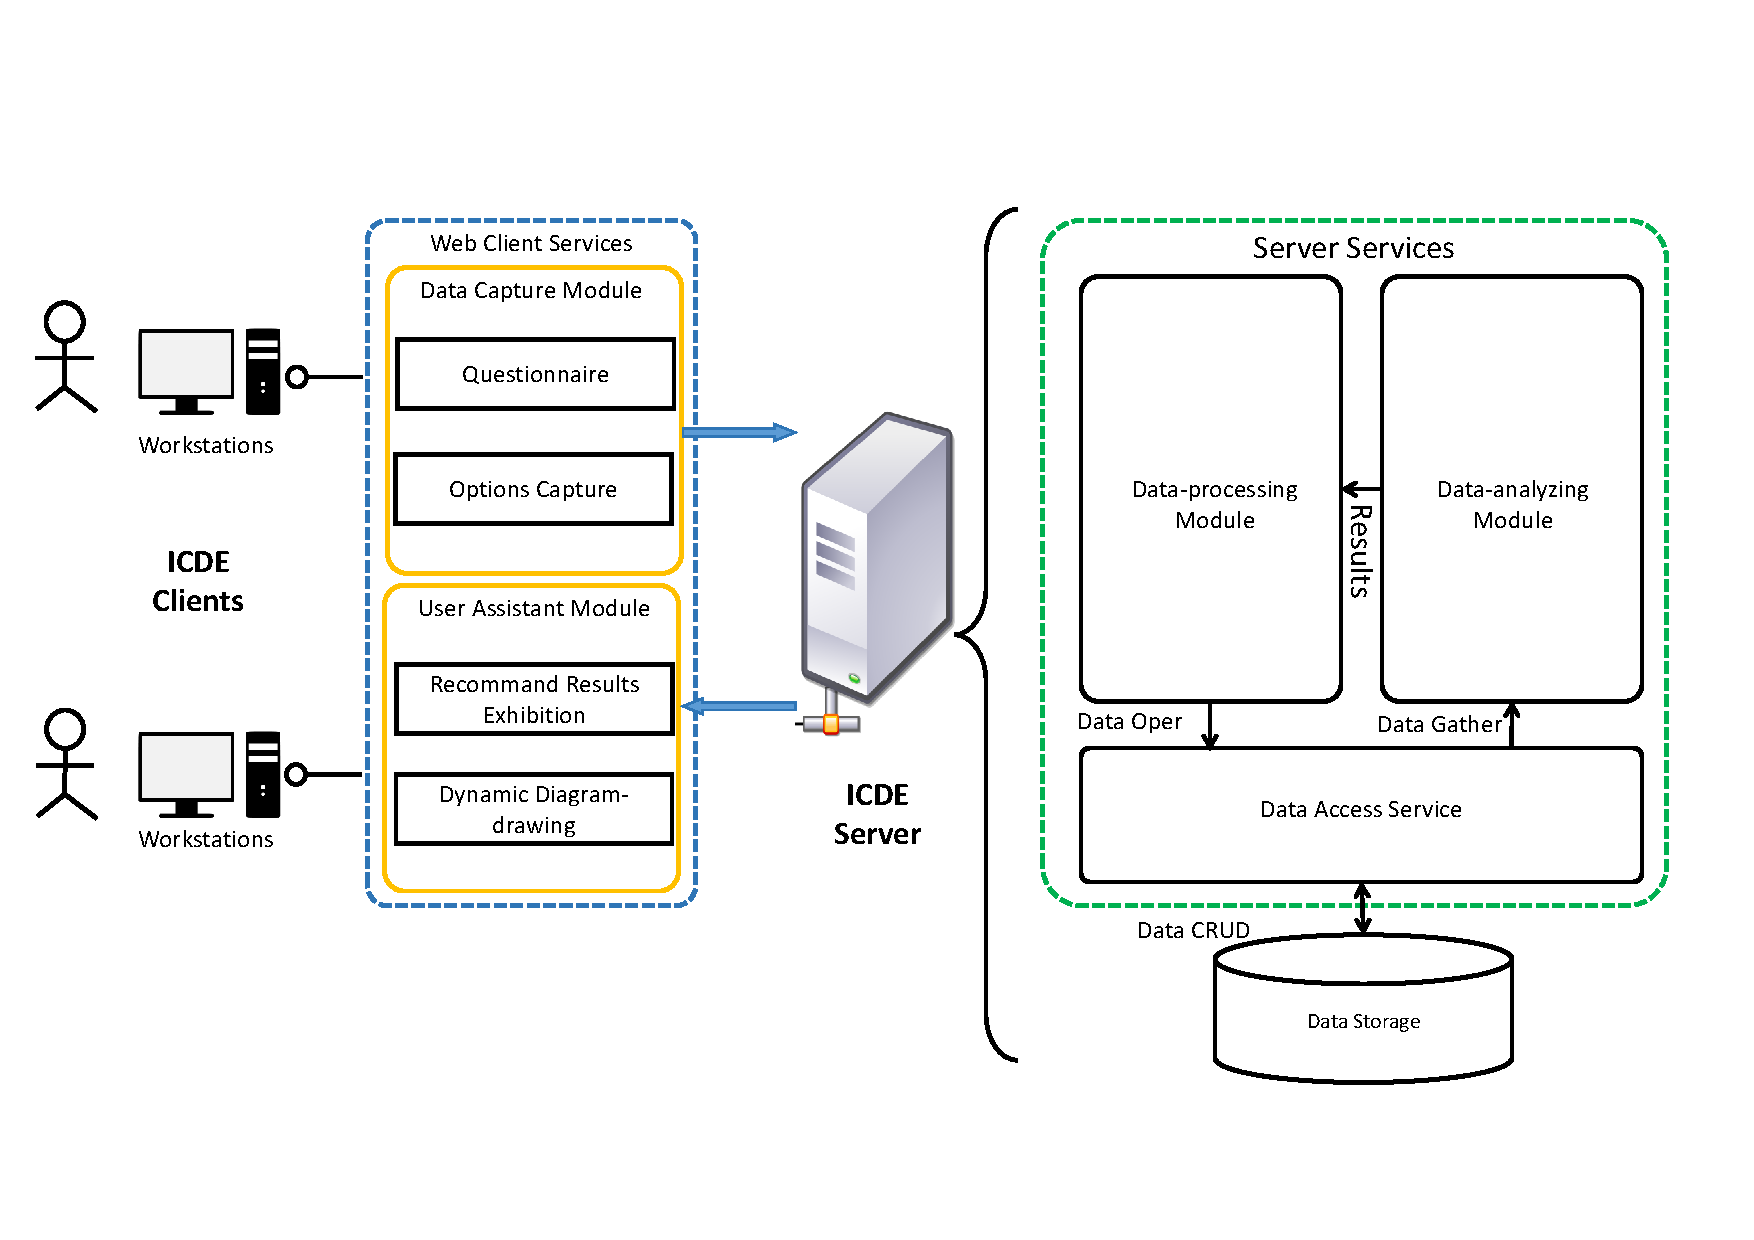
\includegraphics[width=0.9\textwidth]{Architecture.pdf}}
\caption{The architecture graph of Tripedia.}
\label{fig1}
\end{figure*}


\section{\textbf{The Agile Process}}


\subsection{\textbf{Team Setup}}



\subsection{\textbf{Association between User Stories and Sub-requirements}}

\subsection{\textbf{The Scrum Sprint Cycle}}

\subsubsection{\textbf{Review Work to be done}}


\subsubsection{\textbf{Product Backlog}}

\subsubsection{\textbf{Sprint Plan}}



\subsubsection{\textbf{Sprint Backlog}}

\subsubsection{\textbf{Sprint Process}}

\subsubsection{\textbf{Sprint Review}}


\section{\textbf{Architecture}}


\subsection{\textbf{Architecture Design in Overall Level}}

As shown in Figure\ref{fig1}, the ICDE system architecture mainly contains two parts: client and server. Based on the limited server hardware equipment, we implement the data analysis logic as a single module in the server, which stands for ICDE 3rd Party Applications. 

In the client part, we implement Tripedia's client logic based on the web. The web client service is mainly divided into two parts: the Data Capture Module and User Assistant Module. The Data Capture Module captures the user's behavior and personal information through questionnaires and behavior captures, and transmits the relevant information to the server. The User Assistant Module is responsible for displaying processed data sent by the server, such as recommendation results and data analysis results, which help users make decisions easily.

On the server side, we will develop three modules to implement the backbone of the ICDE system: Data-processing Module, Data-analyzing Module, and Data Access Service. The Data Access Service, as the median layer for database access, provides a unified database interface (deletion, modification, query, etc) for the Data-processing Module and the Data-analyzing module. The Data-processing Module is responsible for the basic logic of the server, such as registration, login, search, data preprocessing, and other interaction logic with the client. The Data-analyzing Module accesses the data in the database through the Data Access Service to perform data analysis and returns the analysis results to the Data-processing Module.

To sum up, Tripedia's architecture is a standard ICDE system. The Client part includes a Data Capture Service to collect user behavior and information and transmit relevant data to the server. The Data-processing Module in the Servers section is responsible for implementing the interactive logic of the server; the Data Access Service provides a unified data access interface; the Data-analyzing Module serves as the core of the ICDE system to analyze user data and feedback the analysis results to the user through the server to provide User Assistance Service.


\subsection{\textbf{Architecture Design in User Requirements Level}}



\section{\textbf{Modeling and Design}}


\subsection{\textbf{Task1: Searching data from database }}


\subsubsection{\textbf{Task Conext }}

\begin{figure}[htbp]
	\centerline{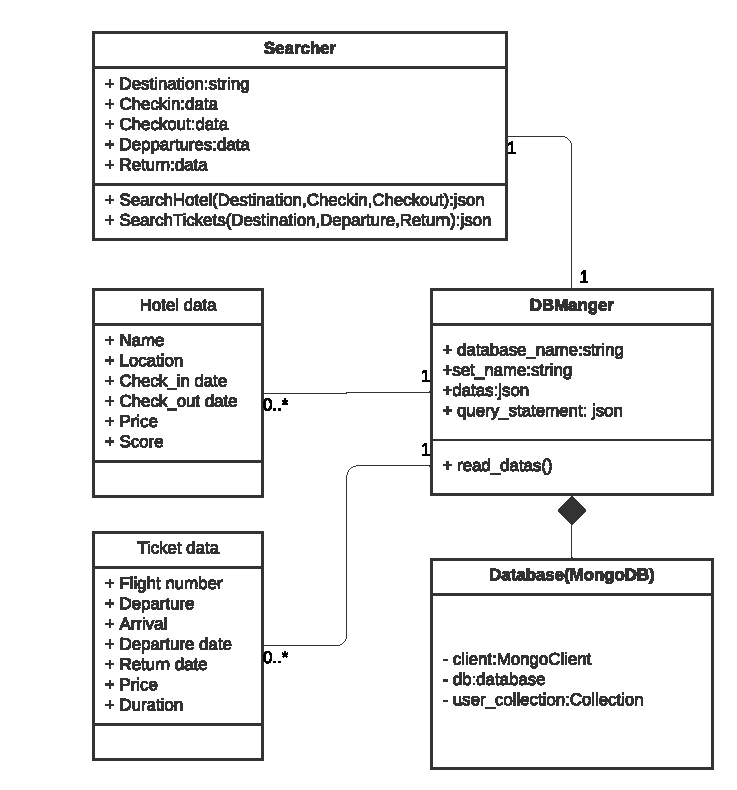
\includegraphics[width=0.4\textwidth]{image/searching hotel class1.pdf}}
	\caption{Class diagram of Searching data from database }
	\label{class1}
\end{figure}

\subsubsection{\textbf{Structural Conext }}

\begin{figure}[htbp]
	\centerline{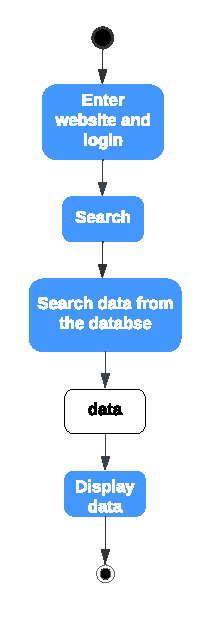
\includegraphics[width=0.4\textwidth]{image/searching hotel activity1.pdf}}
	\caption{Activity diagram of Searching data from database }
	\label{activity1}
\end{figure}


\subsubsection{\textbf{Interaction Conext }}

\begin{figure}[htbp]
	\centerline{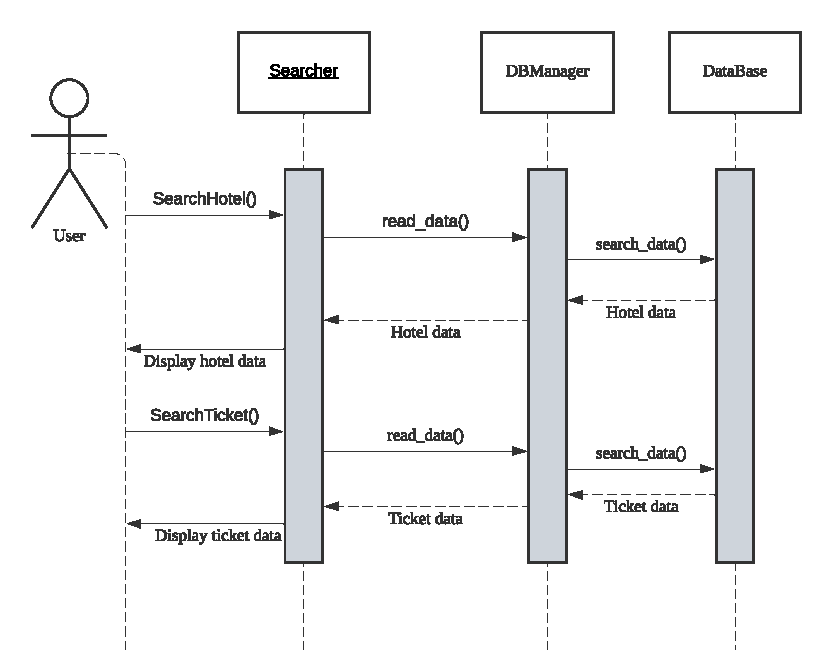
\includegraphics[width=0.4\textwidth]{image/searching hotel sequence1.pdf}}
	\caption{Sequence diagram of Searching data from database }
	\label{sequence1}
\end{figure}

\subsubsection{\textbf{Behavior Conext }}

\begin{figure}[htbp]
	\centerline{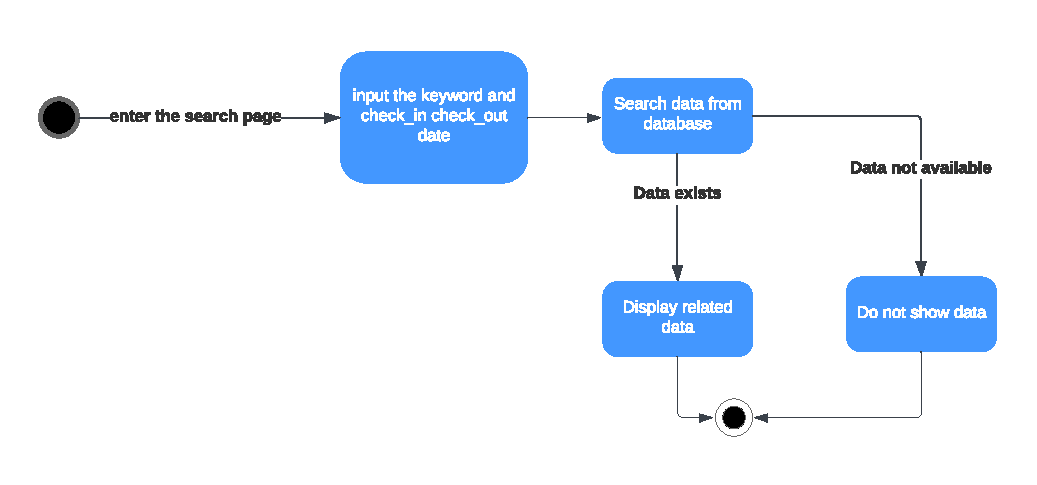
\includegraphics[width=0.4\textwidth]{image/searching hotel statement1.pdf}}
	\caption{Statement diagram of Searching data from database }
	\label{statement1}
\end{figure}

\subsection{\textbf{Task2: Crawler searching }}


\subsubsection{\textbf{Task Conext }}

\begin{figure}[htbp]
	\centerline{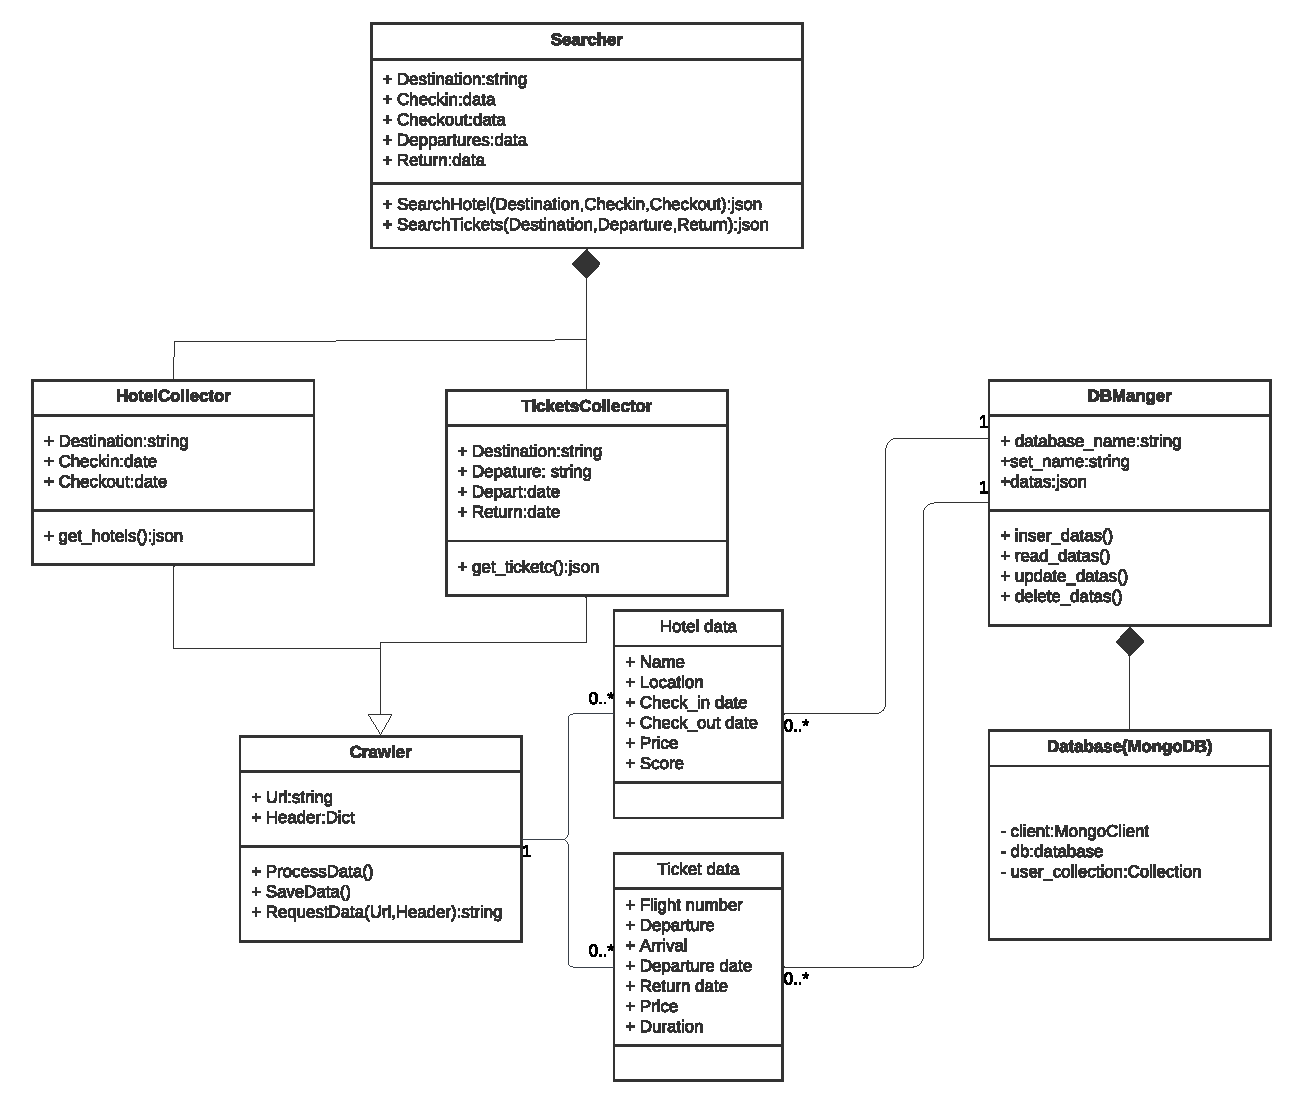
\includegraphics[width=0.4\textwidth]{image/crawler search class1.pdf}}
	\caption{Class diagram of Crawler searching }
	\label{class1}
\end{figure}

\subsubsection{\textbf{Structural Conext }}

\begin{figure}[htbp]
	\centerline{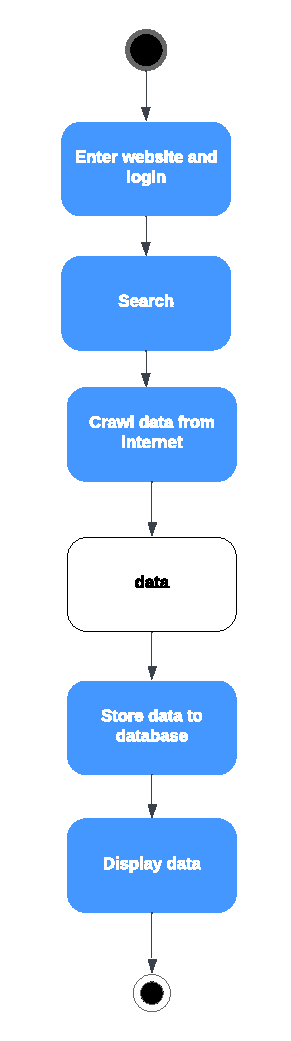
\includegraphics[width=0.4\textwidth]{image/crawler activity1.pdf}}
	\caption{Activity diagram of Crawler searching }
	\label{activity1}
\end{figure}


\subsubsection{\textbf{Interaction Conext }}

\begin{figure}[htbp]
	\centerline{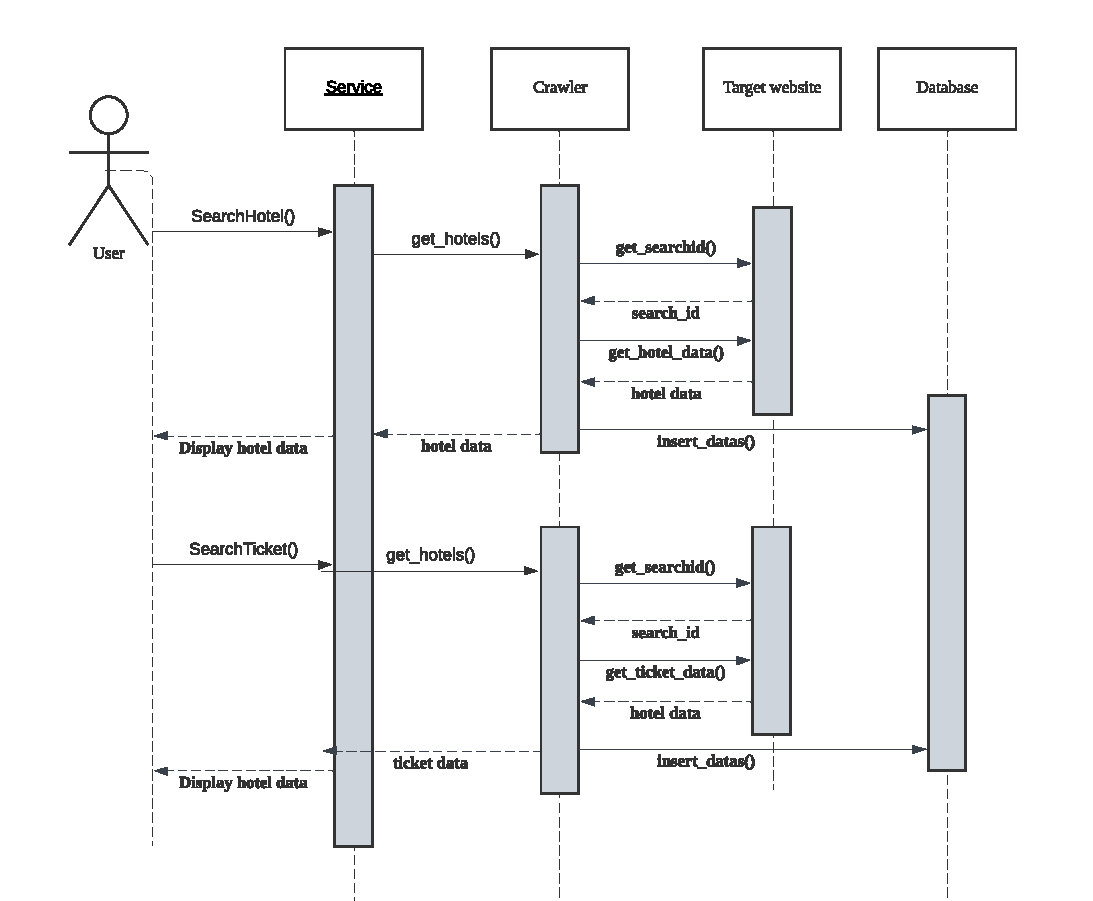
\includegraphics[width=0.4\textwidth]{image/crawler searching sequence1.pdf}}
	\caption{Sequence diagram of Crawler searching }
	\label{sequence1}
\end{figure}

\subsubsection{\textbf{Behavior Conext }}

\begin{figure}[htbp]
	\centerline{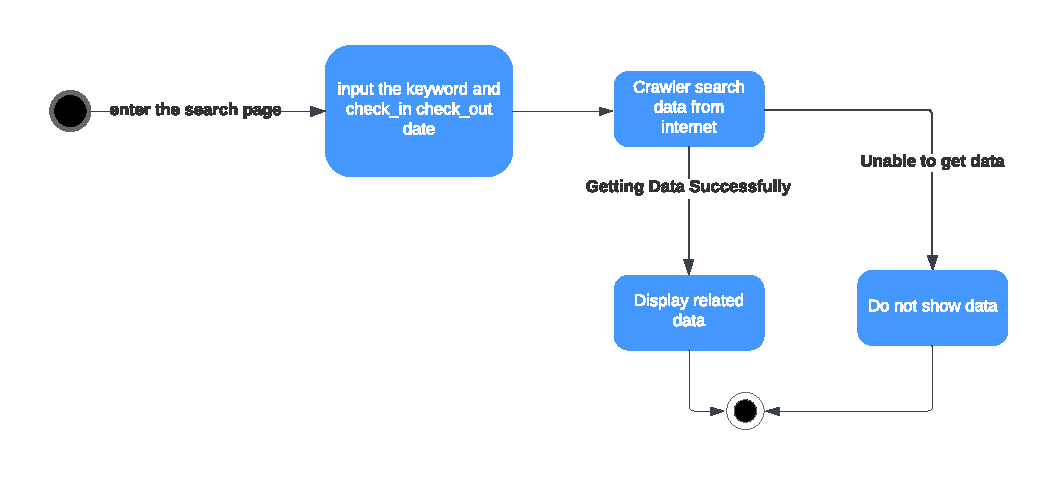
\includegraphics[width=0.4\textwidth]{image/crawler searching statement1.pdf}}
	\caption{Statement diagram of Crawler searching }
	\label{statement1}
\end{figure}


\section{\textbf{Uncompleted Task Design }}


\subsubsection{\textbf{Task Conext }}


\subsubsection{\textbf{Structural Conext }}


\subsubsection{\textbf{Interaction Conext }}


\subsubsection{\textbf{Behavior Conext }}



\section{\textbf{Progress Evaluation \& Analysis }}









\end{document}
